%!TEX root = ..\..\dissertation.tex
\section{Platform Candidate Identification}\label{sec:pltfID}
\cref{paper:APMS2019} is entitled \citetitle{SorensenAPMS2019}, written for and to be presented at the 2019 conference on Advances in Production Management Systems (APMS2019) in September 2019.
It relates to and addresses \cref{resq2} by answering the following sub-question:
\begin{enumerate}[leftmargin=3em]
  \item[RQ2.4] How can a production system classification coding scheme be used to identify candidates for a manufacturing system platform?
\end{enumerate}
This case study applies the classification coding scheme presented by \textcite{SorensenClsfCoding} in an industrial context at the case company.
A classification code is created for a number of manufacturing systems, followed by a comparison and analysis of the resulting code in order to identify potential platform candidates, based on a set of simple drivers and criteria.

\subsection{Extended Abstract}
\subsubsection*{Introduction}
A key aspect of platforms is standardisation of assets.
Standardising tangible and intangible assets of products and manufacturing systems bring platforms their utility in managing variety.
One of the first steps to successful development of manufacturing system platforms is the identification of which assets should or should not be included in a platform~\parencite{SorensenCMS2019}.
Previously, one of the primary sources of \gls{glos:platformCand}s is the tacit knowledge of system experts, who have built up an inherent knowledge on the system of interest~\parencite{SorensenAPMS2018}.
Decisions based on tacit and inherent knowledge can be difficult to communicate and justify to system stakeholders.
A more objective approach to identification of platform candidates can help back up the decisions of system experts.

\Gls{glos:cmmnlty} is frequently the starting point for developing modules and platforms~\parencite{Thevenot2006,Fixson01062007}, but whether similar shapes~\parencite{Cardone2003} or shared assets~\parencite{Kashkoush20161}, commonality can be difficult to find across large, complex systems.
Some progress has been made towards identifying commonality through classification of processes~\parencite{SorensenCMS2018} along with generic and tailored ontologies for integrated product and manufacturing modelling~\parencite{BRUNOE2018592}.
This study builds on top of the classification approach to identifying commonality. 

\subsubsection*{Method}
A production system classification code (PSCC)~\parencite{SorensenClsfCoding} is applied to create a standardised digital representation of the scoped manufacturing systems.
PSCC is a hybrid-code scheme including system design driving requirements, layout, processes and enablers, based on \posscite{SorensenCMS2018} process classification and \posscite{ElMaraghy2006Complexity} manufacturing system complexity coding and classification scheme.
It consists of the 25 digits shown on \cref{fig:PSCC_APMS2019} and is used to create a digital map of a company's production landscape by classifying their existing manufacturing systems.
Digits D1--D9 are filled out once per manufacturing system, while digits D10--D25 are filled out once per process or enabler.
As the code is populated, each digit is given an alphanumeric value with a unique meaning for the specific manufacturing system.
Manufacturing systems are thus represented as grouped strings of alphanumeric values.
\begin{figure}[tb]
  \centering
  \makebox[\textwidth][c]{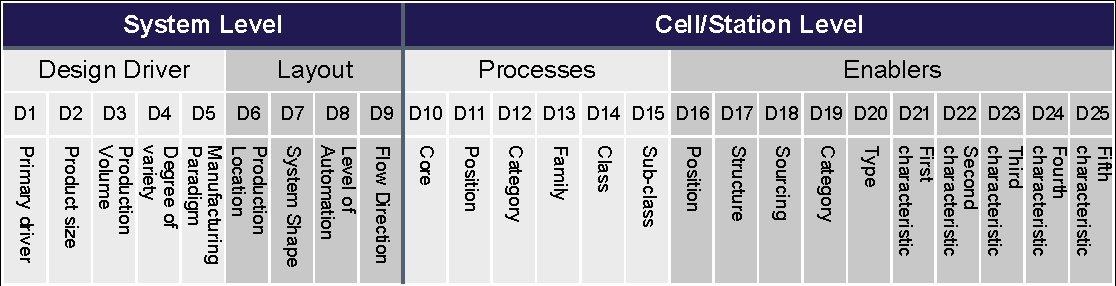
\includegraphics[width=1.1\textwidth, trim=2 2 2 2, clip]{mainmatter/researchResults/figures/PSCC_APMS2019.pdf}}
  \caption[Overview of the production system classification code (PSCC).]
  {Overview of the production system classification coding (PSCC) scheme.
  Adapted from \parencite{SorensenAPMS2019}.}\label{fig:PSCC_APMS2019}
\end{figure}

The populated code for the scoped manufacturing systems will be analysed based on three drivers for \gls{glos:platformCand} identification: (1) frequency, number of instances of a particular process or enabler; (2) prevalence, ratio between number of systems a process or enabler appears in, and the total number of scoped systems; (3) enabler/process ratio, number of different enablers per process and vice versa.
These drivers are examples of reasons why a process or enabler should be a platform candidate, and can be determined by the information captured by the PSCC.

\subsubsection*{Results}
To demonstrate the PSCC and how it can be used to identify \gls{glos:platformCand}s, a case study was carried out with a large Danish manufacturer of discrete products.
Nine distinct manufacturing systems were covered, spanning two departments.
Some systems manufacture components and sub-assemblies for internal use, and others manufacture complete OEM product.
The characteristics of the systems (\eg{} automation level and cycle time) vary greatly, and so do the characteristics of the products (\eg{} product size and features), despite them sharing the same primary function.
All nine systems were surveyed as part of previous projects and case studies, the data from which was used to classify the systems according to the PSCC.

\cref{tab:procSubDri,tab:enaTypeDri} shows the top five process subclasses and top six enabler types ranked according to the previously mentioned platform candidate identification drivers.
21 different process subclasses and 12 different enabler types were covered in the study.
\begin{table}
  \centering
  \caption[Excerpt of the process subclasses ranked by drivers.]
  {Excerpt of the process subclasses ranked by drivers, sorted by total rank~\parencite{SorensenAPMS2019}}\label{tab:procSubDri}
  \small
  \begin{tabular}{lcccccccc}
    \toprule
    \multicolumn{1}{c}{\rotatebox[origin=l]{-90}{\parbox{5em}{Process}}} & \rotatebox[origin=l]{-90}{\parbox{5em}{Frequency}} & \rotatebox[origin=l]{-90}{\parbox{5em}{Frequency rank}} &
    \rotatebox[origin=l]{-90}{\parbox{5em}{Prevalence}} & \rotatebox[origin=l]{-90}{\parbox{5em}{Prevalence rank}} &
    \rotatebox[origin=l]{-90}{\parbox{5em}{Enabler ratio}} & \rotatebox[origin=l]{-90}{\parbox{5em}{Enabler ratio rank}} &
    \rotatebox[origin=l]{-90}{\parbox{5em}{Total score}} & \rotatebox[origin=l]{-90}{\parbox{5em}{Total rank}}\\
    \midrule
    Allocate & 56 & 1 & 1.000 & 1 & 0.089 & 2 & 4 & 1\\
    Screwing & 30 & 2 & 0.556 & 7 & 0.067 & 1 & 10 & 2\\
    Guide & 10 & 4 & 1.00 & 1 & 0.300 & 7 & 12 & 3\\
    Hold & 10 & 4 & 1.00 & 1 & 0.300 & 7 & 12 & 3\\
    Milling \& Routing & 7 & 7 & 0.778 & 4 & 0.286 & 6 & 17 & 5\\
    \ldots \\
    \bottomrule
  \end{tabular}
\end{table}
\begin{table}
  \centering
  \caption[Excerpt of the enabler types ranked by drivers.]
  {Excerpt of the enabler types ranked by drivers, sorted by total rank~\parencite{SorensenAPMS2019}}\label{tab:enaTypeDri}
  \small
  \begin{tabular}{lcccccccccc}
    \toprule
    \multicolumn{1}{c}{\rotatebox[origin=l]{-90}{\parbox{5em}{Process}}} & \rotatebox[origin=l]{-90}{\parbox{5em}{Frequency}} & \rotatebox[origin=l]{-90}{\parbox{5em}{Frequency rank}} &
    \rotatebox[origin=l]{-90}{\parbox{5em}{Prevalence}} & \rotatebox[origin=l]{-90}{\parbox{5em}{Prevalence rank}} &
    \rotatebox[origin=l]{-90}{\parbox{5em}{Process ratio}} & \rotatebox[origin=l]{-90}{\parbox{5em}{Process ratio rank}} &
    \rotatebox[origin=l]{-90}{\parbox{5em}{Enabler ratio}} & \rotatebox[origin=l]{-90}{\parbox{5em}{Enabler ratio rank}} &
    \rotatebox[origin=l]{-90}{\parbox{5em}{Total score}} & \rotatebox[origin=l]{-90}{\parbox{5em}{Total rank}}\\
    \midrule
    Manuel & 89 & 1 & 1.000 & 1 & 0.067 & 1 & 0.067 & 1 & 4 & 1\\
    Conveyor & 11 & 3 & 1.000 & 1 & 0.182 & 5 & 0.273 & 4 & 13 & 2\\
    Pallet & 10 & 4 & 1.000 & 1 & 0.100 & 2 & 0.300 & 7 & 14 & 3\\
    Robot & 23 & 2 & 0.667 & 6 & 0.174 & 4 & 0.261 & 3 & 15 & 4\\
    Mill & 7 & 6 & 0.778 & 5 & 0.143 & 3 & 0.286 & 5 & 19 & 5\\
    Tester & 9 & 5 & 1.000 & 1 & 0.333 & 9 & 0.333 & 8 & 23 & 6\\ 
    \ldots \\
    \bottomrule
  \end{tabular}
\end{table}

The top ranked process in \cref{tab:procSubDri}, allocate, is a material handling process defined as the creation of a defined partial quantity of parts and the movement of the same quantity to a target location~\parencite{SorensenCMS2018}.
With an apparent low variety of enablers and high prevalence and frequency, a platform for the allocate process likely already exists, or there is an agreed upon way to carry out the process.
If the former is the case, the platform should be documented, and in the case of the latter, a platform should be developed.
In either case, the process is a clear \gls{glos:platformCand}.

The second highest ranked process, screwing, is a manufacturing process.
While it ranks low in terms of prevalence (rank 7), it has a low variety and high frequency.
Once again, the classification and analysis indicates that a standardised way to carry out the process exists, and that it should be developed and formally described as a platform.

As for enablers, manual is ranked first by quite a margin.
The manual enabler represents an operator in the system being the impetus behind a process.
Alongside the conveyor, pallet and tester, it appears in all scoped systems.
Due to their high prevalence (1.000), all four show potential for platform development, while both the pallet, and tester also show room for improved standardisation with a relatively high enabler ratio for their prevalence (0.300 and 0.333 respectively).
Lastly, the robot enabler is a clear candidate, ranking second in frequency and performing four different processes using six distinct enablers.

\subsubsection*{Conclusions}
Nine previously surveyed manufacturing systems were classified according to a production system classification coding scheme, with the intention of comparing the manufacturing systems to identify commonality and thus potential platform candidates.
The classification coding scheme captures key characteristics of the manufacturing systems, including its driving requirements, structure, and functions.
Based on this, potential \gls{glos:platformCand}s in the form of processes and enablers can be identified and ranked according to a number of drivers indicating their suitability for platform development.
Both the PSCC and ensuing comparison of the populated code act as decision support tools for manufacturers looking towards brownfield platform development.

\subsection{Implications}
The study presented above takes the next step in supporting platform development by demonstrating how a decision support tool can be used to identify new platform candidates.
Implementation of the classification coding scheme within a company remains a challenge, and there is a need for a concrete, dedicated application facilitating creation of the code in an intuitive manner.

Several changes can be made to strengthen the platform identification approach based on the PSCC.
An obvious way to do so, is to include additional drivers and digits for ranking the various processes and enablers, for instance using digit D10 to determine how many instances of a process are considered ``core'' to the manufacturer.
Performance and cost data can also be included to help separate ``good'' and ``bad'' solutions, \ie{} solutions with good performance and low cost versus bad performance and high costs.
This could also potentially let manufacturers determine a correlation between characteristics of a system or enabler and its cost and performance.
Summing up, the contributions made through the study are listed below:
\begin{enumerate}
  \item Applies \posscite{SorensenClsfCoding} classification coding scheme to show its feasibility.
  \item Highlights the difficulty inherent to implementing a classification coding scheme in an industrial context.
  \item Demonstrates how potential platform candidates can be identified using a classification coding scheme.
 \end{enumerate}